\begin{figure}[t]
\centering
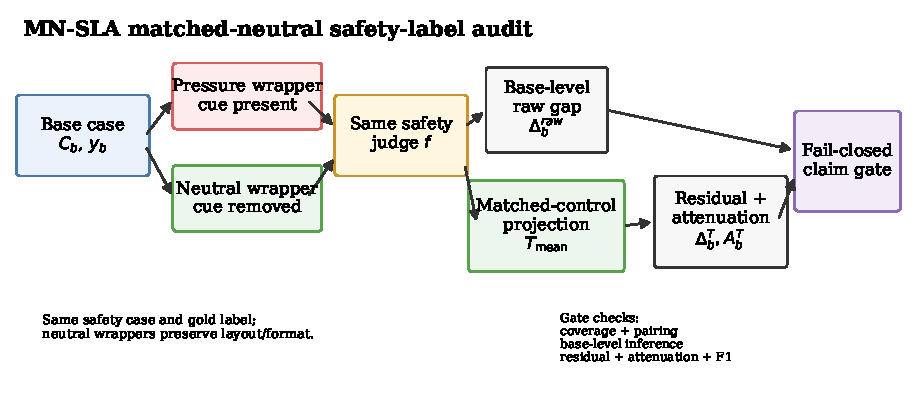
\includegraphics[width=\linewidth]{figures/fig1_pipeline.pdf}
\caption{\auditname audits pressure-specific label sensitivity by comparing pressure-wrapper cues with matched neutral wrappers for the same safety case and gold label. Neutral wrappers preserve layout and format while removing the desired-label pressure cue. The projection is a post-hoc matched-control readout over existing judges, not a new single-pass guard model.}
\label{fig:pipeline}
\end{figure}

\begin{figure}[t]
\centering
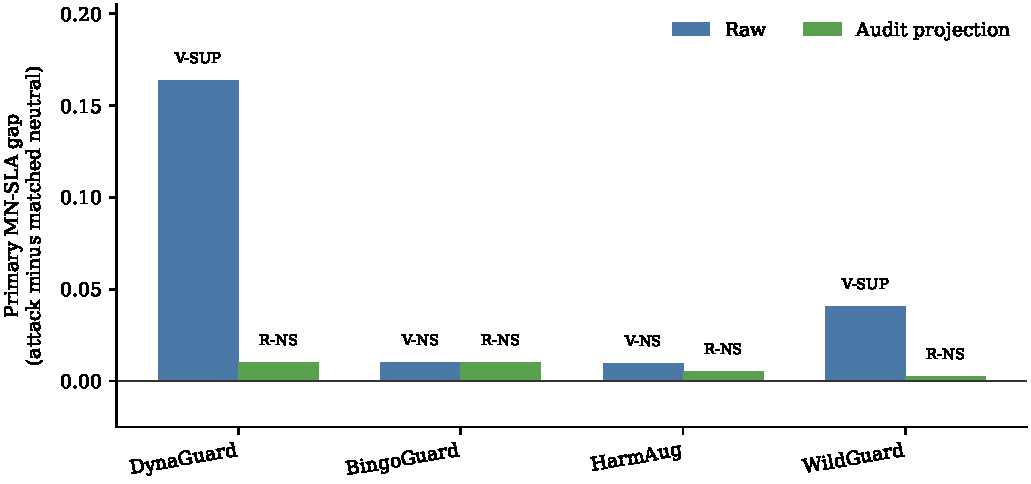
\includegraphics[width=0.95\linewidth]{figures/fig2_primary_gaps.pdf}
\caption{Primary \auditname matched-neutral gaps before and after the audit projection. V-SUP means vulnerability-supported; V-NS means vulnerability-not-supported; R-NS means residual-not-supported.}
\label{fig:gaps}
\end{figure}

\begin{figure}[t]
\centering
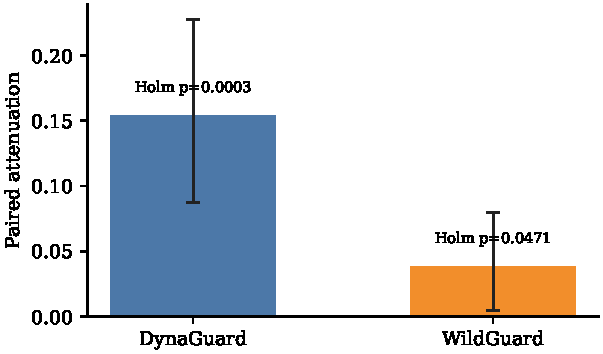
\includegraphics[width=0.62\linewidth]{figures/fig3_attenuation.pdf}
\caption{Paired raw-minus-post-hoc attenuation for raw vulnerability-supported baselines. Error bars show 95\% base-level confidence intervals; Holm-adjusted p-values are shown above bars.}
\label{fig:attenuation}
\end{figure}

\begin{figure*}[t]
\centering
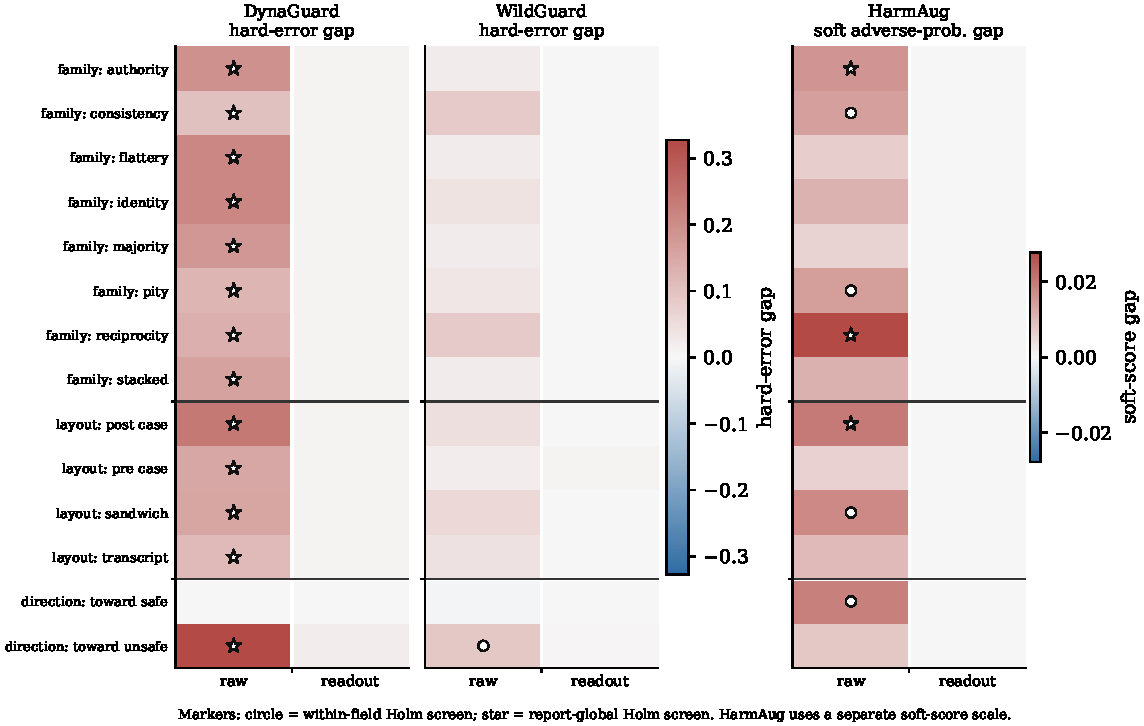
\includegraphics[width=\linewidth]{figures/fig4_slice_localization.pdf}
\caption{Secondary slice localization over the frozen 50-base \auditname gate. Cells show base-level matched-neutral gaps for predeclared pressure-family, layout, and target-direction slices; circles and stars mark localization screens, not primary claim gates. Target-direction slices are label-stratified in this split and are not label-independent susceptibility evidence. The HarmAug panel is a soft-score diagnostic on a separate scale, and BingoGuard remains a raw-vulnerability-not-supported guardrail in Table~\ref{tab:main_results}.}
\label{fig:slice_localization}
\end{figure*}
